\documentclass[12pt]{article}
\usepackage[margin=0.9in]{geometry} 
\usepackage{amsmath}
\usepackage{tcolorbox}
\usepackage{hyperref}
\usepackage{amssymb}
\usepackage{amsthm}
\usepackage{graphicx}
\usepackage{lastpage}
\graphicspath{ {./} }
\usepackage{fancyhdr}
\usepackage{accents}
\pagestyle{fancy}
\setlength{\headheight}{40pt}


\newenvironment{solution}
  {\renewcommand\qedsymbol{$\blacksquare$}
  \begin{proof}[Solution]}
  {\end{proof}}
\renewcommand\qedsymbol{$\blacksquare$}

\newcommand{\ubar}[1]{\underaccent{\bar}{#1}} % add packages, settings, and declarations in settings.tex


\begin{document}

\lhead{Crețu Cristian} 
\rhead{clasa a XII-a} 
\cfoot{\thepage\ din \pageref{LastPage}}


\textbf{\LARGE Detecția în infraroșu
}

\vspace{0.5cm}
Radiația în infraroșu (IR) este o radiație electromagnetică a cărei lungime de undă este mai lungă decât cea a luminii vizibile (400 - 700 nm), dar mai scurtă decât cea a radiației terahertz (100 μm - 1 mm) și a microundelor (30000 μm). Majoritatea radiației termice emise de către obiectele aflate la temperatura camerei este în infraroșu.\footnote{Wikipedia - Infraroșu}

Ochii noștri sunt detectori proiectați pentru a observa spectrul de lumină (radiații) vizibilă. Insă, putem vedea doar o mică parte din gama de radiații numite spectrul electromagnetic.

\begin{figure}[h]
    \centering
    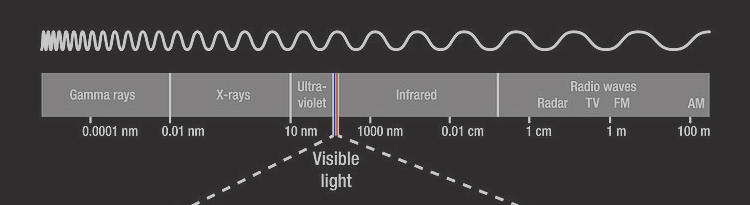
\includegraphics[width=0.9\textwidth]{electro.jpg}
    \caption{Spectrul Electromagnetic}
    \label{fig:mesh1}
\end{figure}

Radiația infraroșie începe la marginea vizibilă a spectrului, mai exact de la extremitatea culorii roșii de la 700nm, până la 1mm. Această limită de lungime de undă corespunde frecvenței cuprinse între 430 THz până la 300GHz.

\section{Senzor IR pasiv}

\quad \quad Senzorul infraroșu pasiv este un dispozitiv electronic care măsoară radiația infraroșie emisă de obiecte aflate în câmpul său vizual. Este mai ales folosit în construcția detectoarelor de mișcare. 
\footnote{Wikipedia - Senzor infraroșu pasiv}

\quad Toate corpurile emit energie sub formă de radiații. Radiațiile infraroșii sunt invizibile pentru ochiul uman, dar pot fi detectate de dispozitive electronice concepute în acest sens.

\begin{figure}[!h]
    \centering
    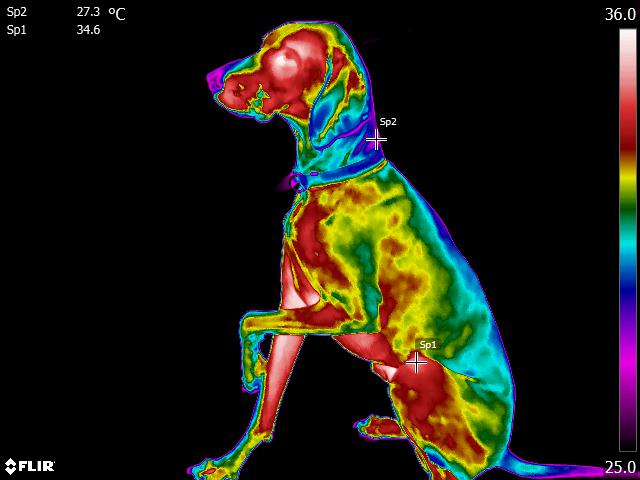
\includegraphics[width=0.4\textwidth]{dog.jpg}
    \caption{Exemplu - un câine în IR}
    \label{fig:mesh1}
\end{figure}

\quad Un detector de mișcare este un dispozitiv de recunoaștere a mișcărilor de corpuri (obiecte, persoane) în vecinătatea lui. Un astfel de detector conține un mecanism fizic sau un senzor electronic care cuantifică mișcarea și care poate să fie integrat sau conectat la alte dispozitive care să alerteze utilizatorul de prezența unui obiect în mișcare în raza de acțiune a senzorului. Detectoarele de mișcare sunt o componentă vitală a sistemelor de securitate atât pentru locuințe cât și pentru firme.

\quad Astfel, un senzor pasiv în infraroșu (senzor PIR) este un dispozitiv electronic care măsoară radiația infraroșie (IR) provenită de la obiecte aflate în câmpul său vizual. Mișcarea este detectată atunci când un corp cu o anumită temperatură (cum ar fi un om sau un animal) trece prin fața sursei infraroșu cu o altă temperatură, cum ar fi un perete. Acest lucru înseamnă că senzorul detectează căldura de la trecerea unui obiect prin câmpul de acțiune al senzorului și acel obiect rupe câmpul pe care senzorul l-a determinat anterior ca fiind “normal”. Orice obiect, chiar unul de aceeași temperatură ca și obiectele din jur va activa senzorul PIR dacă corpul se deplasează în câmpul vizual al senzorului. Senzorul (de mișcare) cu infraroșu nu răspunde la diferențele termice statice, care sunt cauzate prin mijloace naturale cum ar fi expunerea la lumina soarelui.

\quad În fața senzorului propriu-zis - în distanța focală - se găsește o cupolă sferică sau cilindrică de lentile mici curbe convexe albe, din material plastic noros, dar este în mod clar în infraroșu transparent. Aceste lentile multiple colectează lumină în infraroșu. Lumina în infraroșu ajunge la senzorul propriu-zis care transformă această energie infraroșie în energie electrică, care poate fi analizată de un circuit de procesare (procesor) și care va diferenția alarmele false de alarmele reale.

\section{Cum funcționează?}

\quad Detecția în infraroșu utilizează o varietate de materiale pentru a crea o reacție care răspunde la radiațiile electromagnetice. Senzorul va combina un strat de telurură de cadmiu și mercur, un strat de sulfură de plumb și un strat de antimonitură de indiu în substrat de siliciu. Metalele creează un semiconductor în cadrul dispozitivului. Sensibilitatea se bazează pe faptul că dispozitivul emite radiații sau le absoarbe. Lumina este transformată în interiorul structurii într-un curent electric. Lumina emite fotodiode, ceea ce înseamnă că lumina emite lungimi de undă spectrale care pot fi interpretate ca un semnal electric. În funcție de tipul de senzor, acesta poate fi interpretat într-un aparat de termoviziune, un interval de temperatură, un detector de mișcare sau o cameră LWIR. \footnote{covesmart.com/blog/infrared-detector/}

\section{Exemple practice}

Datorită stării de echilibru termic, două corpuri vor tinde spre o temperatură mediană. (Corpul cald pierde căldura, cel rece o primește). Astfel, la un POS, o captură în IR este capabilă de a determina în 80 din cazuri PIN-ul. (Observăm atât cifrele apăsate, cât și ordinea apăsării, datorită schimbului de căldură - cel mai cald buton este apăsat ultimul, etc.) \footnote{cseweb.ucsd.edu/~kmowery/papers/thermal.pdf}

\begin{figure}%
    \centering
    \subfloat[\centering PIN = 12345]{{ 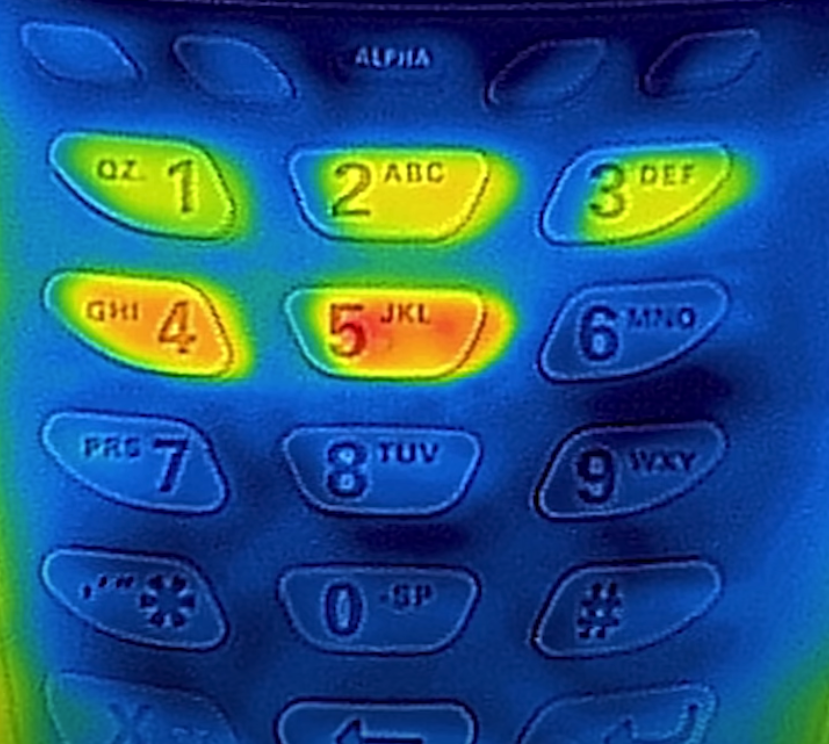
\includegraphics[width=0.3\textwidth]{pin.png} }}%
    \qquad
    \subfloat[\centering Metalul reflecta undele IR]{{ 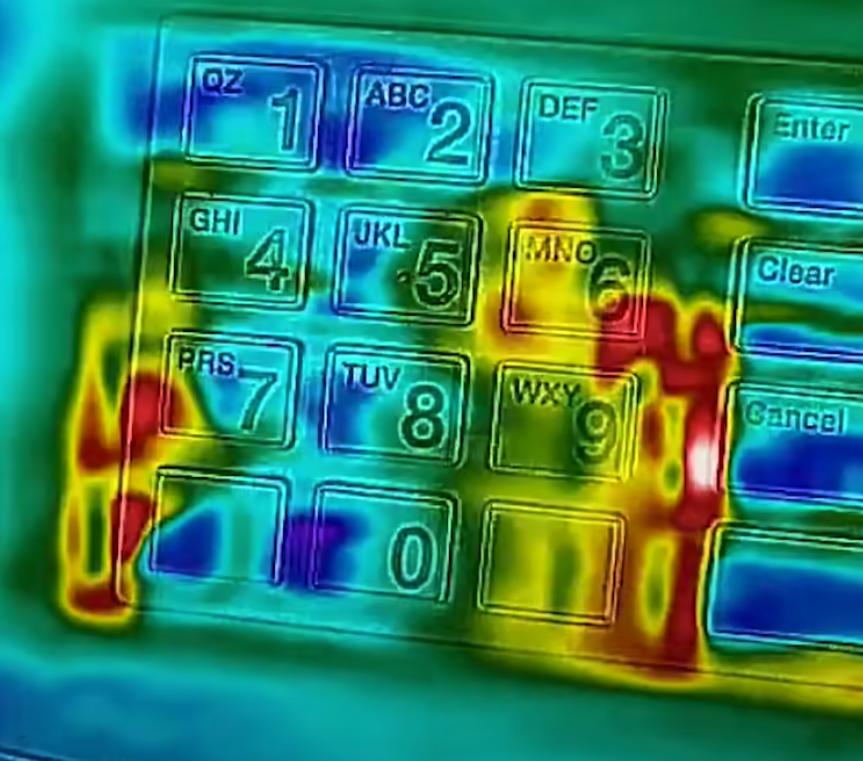
\includegraphics[width=0.3\textwidth]{atm.png} }}%
    \caption{PIN în IR, plastic vs. metal}%
    \label{fig:example}%
\end{figure}

\begin{figure}%
    \centering
    \subfloat[\centering Urmă pe drum]{{ 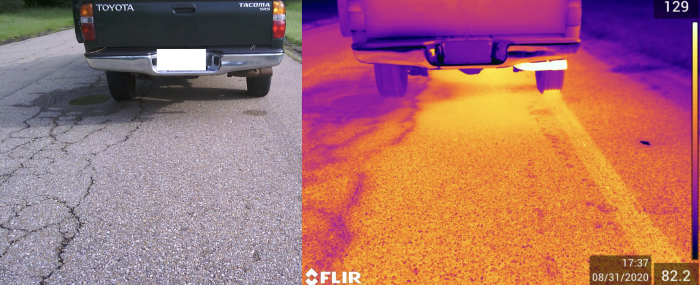
\includegraphics[width=0.5\textwidth]{frecare.png} }}%
    \qquad
    \subfloat[\centering Urmă pe discul de frână]{{ 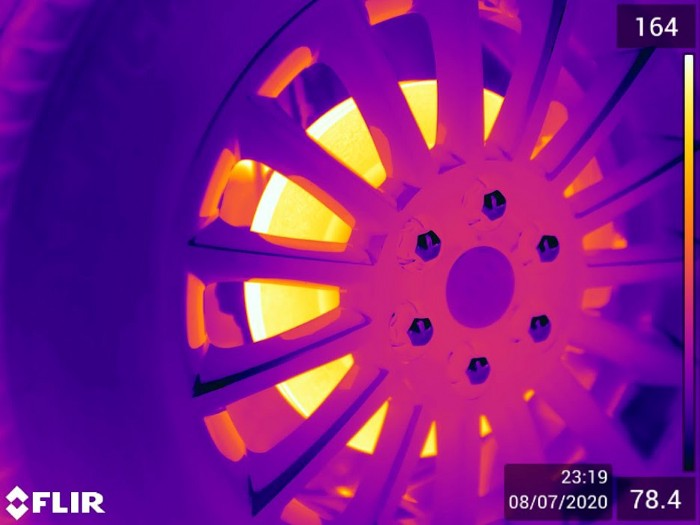
\includegraphics[width=0.3\textwidth]{brake.jpg} }}%
    \caption{Urmele forței de frecare}%
    \label{fig:example}%
\end{figure}

\begin{figure}%
    \centering
    \subfloat[\centering Bec incandescent vs. LED]{{ 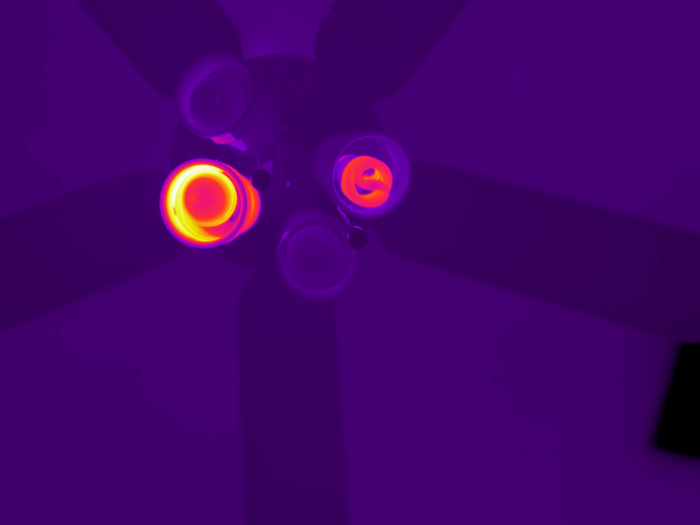
\includegraphics[width=0.4\textwidth]{bec.png} }}%
    \qquad
    \subfloat[\centering Prelungitor]{{ 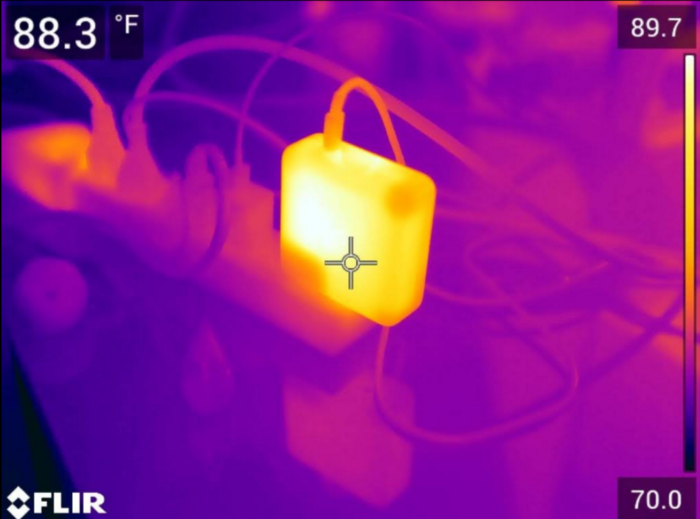
\includegraphics[width=0.4\textwidth]{curent.png} }}%
    \caption{În electricitate}%
    \label{fig:example}%
\end{figure}


\end{document}
